\newpage
\section{SVPWM调制技术}
\subsection{SVPWM基本分析}

经过第一章的分析，可以发现，在同步旋转坐标系下对电机进行分析是非常简单的。但是
同步旋转坐标系的电压\(U_{\mathrm{d}},U_{\mathrm{q}}\)是一种数学变量，其并不真实可控。大部分永磁同步电机
控制电路为下图所示的三相全桥逆变电路，能被直接控制的只有自然坐标系下的三相电压
\(U_{\mathrm{a}},U_{\mathrm{b}},U_{\mathrm{c}}\)，因此如何将希望得到的\(U_{\mathrm{d}},U_{\mathrm{q}}\)，转换为可以直接控制的
\(U_{\mathrm{a}},U_{\mathrm{b}},U_{\mathrm{c}}\)，就是调制技术关注的点。
\begin{figure}[H]
    \centering
    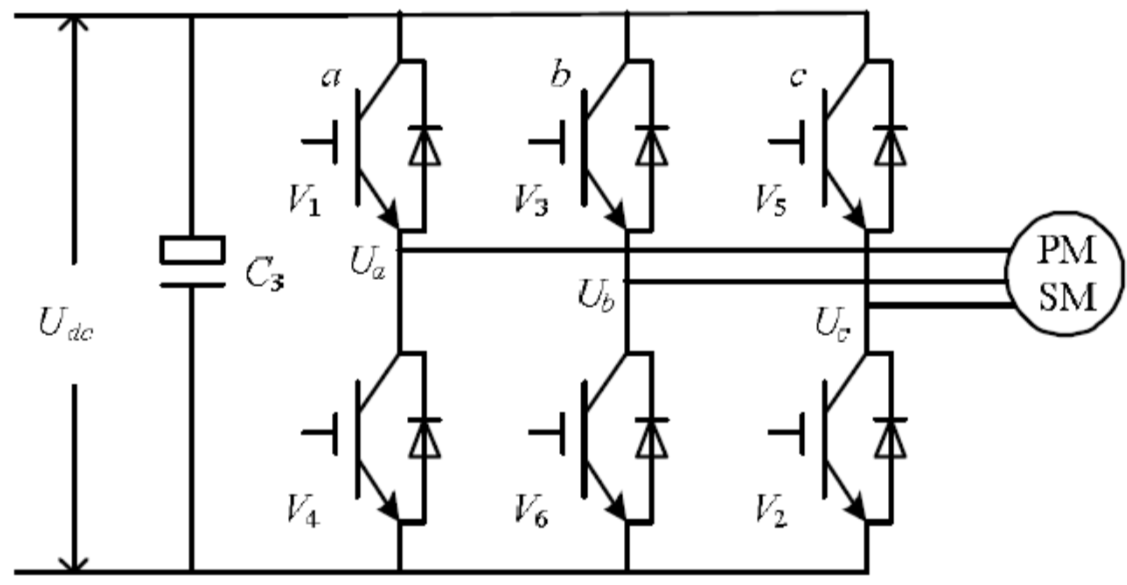
\includegraphics[width=0.4\textwidth]
    {图片/三相全桥逆变电路.png}
    \caption{三相全桥逆变电路}
    \label{fig:三相全桥逆变电路}
\end{figure}

SVPWM（Space Vector Pulse Width Modulation，空间矢量脉宽调制）
是一种针对三相全桥的PWM调制技术，其基本思想是将希望得到的电压矢量用多个基本矢量
来合成。基本矢量可以用\(U_{\mathrm{x}}(S_{\mathrm{A}},S_{\mathrm{B}}, S_{\mathrm{C}})\)表示，其中\(S_{\mathrm{A}},S_{\mathrm{B}},S_{\mathrm{C}}\)为三相全桥的
开关状态，而\(x=4S_{\mathrm{A}}+2S_{\mathrm{B}}+S_{\mathrm{C}}\)为基本矢量的索引。
如A相导通，B、C相截止，就可以表示为\(U_4(1,0,0)\)。

根据三相全桥各相的开关状态，基本矢量可以分为两种有效矢量和两种零矢量共四类。

第一种有效矢量包括\(U_4(1,0,0),U_2(0,1,0),U_1(0,0,1)\)三个基本矢量，特点是单相
上桥导通、两相下桥截止。此时导通的上桥流过的电流就是母线电流。

第二种有效矢量包括\(U_3(0,1,1),U_5(1,0,1),U_6(1,1,0)\)三个基本矢量，特点是两相
上桥导通、一相下桥截止。此时导通的下桥流过的电流就是母线电流。

另外还有两种零矢量为\(U_0(0,0,0)\)和\(U_7(1,1,1)\)，分别是三相截止和三相导通。
此时通过MOSFET、IGBT等功率器件的寄生/续流二极管形成环流。

将上述的基本矢量在两相静止坐标系种表示如下图所示。可以发现，平面被八个基本电压
矢量分割为了六个扇区。
\begin{figure}[H]
    \centering
    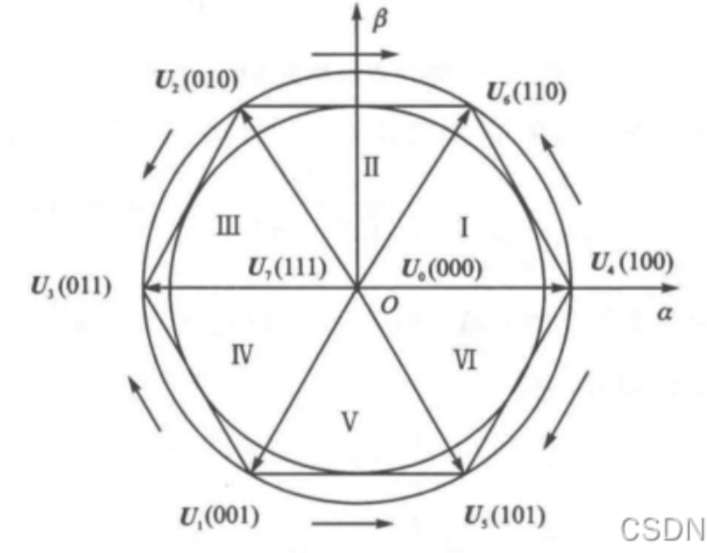
\includegraphics[width=0.6\textwidth]
    {图片/SVPWM基本矢量和扇区划分图.png}
·    \caption{SVPWM基本矢量和扇区划分图}
    \label{fig:SVPWM基本矢量和扇区划分图}
\end{figure}

根据等幅值克拉克变换\eqref{eq:克拉克变换}可得基本矢量幅值为
\(\cfrac{2}{3}U_{\mathrm{dc}}\)。
根据合成矢量的规则，任一电压矢量都可以用相邻60°的两个基本矢量和零矢量得到

接下来以第I扇区为例，讨论合成矢量的幅值要求。第I扇区可以使用有效矢量
\(U_4(1,0,0)\)和\(U_6(1,1,0)\)与零矢量\(U_0(0,0,0)\)和\(U_7(1,1,1)\)。
为了获取最大的电压矢量，假设零矢量不参与合成。在一个PWM周期内，\(k\)时间占比
由\(U_4(1,0,0)\)作用，而\(1-k\)时间占比由\(U_6(1,1,0)\)作用。

用复数表示合成矢量，则合成矢量可以表示为
\(U=\cfrac{2}{3}U_{\mathrm{dc}}(k+\cfrac 12(1-k)+\mathrm{j}\cfrac{\sqrt{3}}{2}(1-k))\)
，其中j表示虚数单位。该合成矢量的幅值为
\(\cfrac{2}{3}U_{\mathrm{dc}}\sqrt{(k+\cfrac 12-\cfrac 12k)^2+\cfrac 34(1-k)^2}
=\cfrac 23U_{\mathrm{dc}}\sqrt{k^2-k+1}\)
，其中作用时间占比\(k\in [0,1]\)。

根据二次函数相关知识可得当\(k=\cfrac 12\)时合成矢量幅值最小，此时合成矢量
幅值为\(\cfrac{1}{\sqrt 3}U_{\mathrm{dc}}\)。这就是可以完成线性调制的SVPWM电压极限圆
半径（正六边形内切圆）。在电压极限圆内，任何电压矢量都可以用基本矢量合成得到。
而超出电压极限圆范围，但只要处于正六边形范围内，也都可以用基本矢量合成得到。

由于正六边形范围的判断较为复杂，因此一般认为SVPWM的调制极限就是电压极限圆，
也即满足
\begin{equation}
    U_{\mathrm{d}}^2+U_{\mathrm{q}}^2\le \cfrac{U_{\mathrm{dc}}^2}{3}
    \label{eq:SVPWM电压极限圆}
\end{equation}

根据电压极限圆可知，SVPWM调制法的相电压最大利用率为
\(\cfrac{\frac{U_{\mathrm{dc}}}{\sqrt 3}}{U_{\mathrm{dc}}}\times100\%=57.7\%\)，
而线电压最大利用率为
\(\sqrt{3}\times \cfrac{\frac{U_{\mathrm{dc}}}{\sqrt 3}}{U_{\mathrm{dc}}}
\times100\%= 100\%\)。

\subsection{SVPWM调制法}
\label{sec:SVPWM调制法}

SVPWM调制法是基本的SVPWM实现方法，其物理含义直观，但是程序运行效率较低，
这是因为需要经过扇区判断、基本矢量作用时间计算、三相占空比计算三个步骤。

扇区判断的主要任务是，将给定的\(U_{\mathrm{d}},U_{\mathrm{q}}\)，通过\eqref{eq:帕克逆变换}的帕克
逆变换公式得到两相静止坐标系下的\(U_{\mathrm{\alpha}},U_{\mathrm{\beta}}\)，判断合成矢量
所在的扇区。

根据基本矢量图\ref{fig:SVPWM基本矢量和扇区划分图}，可以得到合成矢量
落在特定扇区的充要条件。
\begin{itemize}
    \item 
    扇区I：\(U_{\mathrm{\alpha}}>0,{U_{\mathrm{\beta}}>0},
    |\cfrac{U_{\mathrm{\beta}}}{U_{\mathrm{\alpha}}}|<\sqrt 3\)
    第三个条件也可以写为
    \(\begin{cases}\cfrac 12(\sqrt{3}U_{\mathrm{\alpha}}-U_{\mathrm{\beta}})>0\\
        \cfrac 12(-\sqrt{3}U_{\mathrm{\alpha}}-U_{\mathrm{\beta}})<0\end{cases}\)
    \item 
    扇区II：\({U_{\mathrm{\beta}}>0},|\cfrac{U_{\mathrm{\beta}}}{U_{\mathrm{\alpha}}}|>\sqrt 3\)
    第三个条件也可以写为
    \(\begin{cases}\cfrac 12(\sqrt{3}U_{\mathrm{\alpha}}-U_{\mathrm{\beta}})<0\\
        \cfrac 12(-\sqrt{3}U_{\mathrm{\alpha}}-U_{\mathrm{\beta}})<0\end{cases}\)
    \item 
    扇区III：\(U_{\mathrm{\alpha}}<0,{U_{\mathrm{\beta}}>0},
    |\cfrac{U_{\mathrm{\beta}}}{U_{\mathrm{\alpha}}}|<\sqrt 3\)
    第三个条件也可以写为
    \(\begin{cases}\cfrac 12(\sqrt{3}U_{\mathrm{\alpha}}-U_{\mathrm{\beta}})<0\\
        \cfrac 12(-\sqrt{3}U_{\mathrm{\alpha}}-U_{\mathrm{\beta}})>0\end{cases}\)
    \item 
    扇区IV：\(U_{\mathrm{\alpha}}<0,{U_{\mathrm{\beta}}<0},
    |\cfrac{U_{\mathrm{\beta}}}{U_{\mathrm{\alpha}}}|<\sqrt 3\)
    第三个条件也可以写为
    \(\begin{cases}\cfrac 12(\sqrt{3}U_{\mathrm{\alpha}}-U_{\mathrm{\beta}})<0\\
        \cfrac 12(-\sqrt{3}U_{\mathrm{\alpha}}-U_{\mathrm{\beta}})>0\end{cases}\)
    \item 
    扇区V：\({U_{\mathrm{\beta}}<0},|\cfrac{U_{\mathrm{\beta}}}{U_{\mathrm{\alpha}}}|>\sqrt 3\)
    第三个条件也可以写为
    \(\begin{cases}\cfrac 12(\sqrt{3}U_{\mathrm{\alpha}}-U_{\mathrm{\beta}})>0\\
        \cfrac 12(-\sqrt{3}U_{\mathrm{\alpha}}-U_{\mathrm{\beta}})>0\end{cases}\)
    \item 
    扇区VI：\(U_{\mathrm{\alpha}}>0,{U_{\mathrm{\beta}}<0},
    |\cfrac{U_{\mathrm{\beta}}}{U_{\mathrm{\alpha}}}|<\sqrt 3\)
    第三个条件也可以写为
    \(\begin{cases}\cfrac 12(\sqrt{3}U_{\mathrm{\alpha}}-U_{\mathrm{\beta}})>0\\
        \cfrac 12(-\sqrt{3}U_{\mathrm{\alpha}}-U_{\mathrm{\beta}})<0\end{cases}\)
\end{itemize}

可以发现上述条件判断都可以用
\(\begin{cases}A_0=U_{\mathrm{\beta}}
    \\A_1=\cfrac{\sqrt{3}}2U_{\mathrm{\alpha}}-\cfrac{1}{2}U_{\mathrm{\beta}}
    \\A_2=-\cfrac{\sqrt{3}}2U_{\mathrm{\alpha}}-\cfrac 12U_{\mathrm{\beta}}
\end{cases}\)
的符号判断来概括。若定义上述判断式结果大于零为真（1），小于零为假（0），
也就是满足\(X_i=\begin{cases}1&A_i>0\\0&A_i<0\end{cases}\)
则可以定义逻辑向量\((X_2,X_1,X_0)\)，索引值为\(N'=4X_2+2X_1+X_0\)。索引值的
可取值为\(1,2,3,4,5,6\)，分别对应六种扇区，记扇区号为\(N\)，判断表如下。
\begin{table}[H]
    \centering
    \begin{tabular}{|c|c|c|c|}
        \hline
        扇区号N&充要条件&逻辑向量&索引值N'\\
        \hline
        I&
        \(\begin{cases}-\sqrt{3}U_{\mathrm{\alpha}}-U_{\mathrm{\beta}}<0\\
            \sqrt{3}U_{\mathrm{\alpha}}-U_{\mathrm{\beta}}>0\\
            U_{\mathrm{\beta}}>0\end{cases}\)&
        (0,1,1)&3\\
        \hline
        II&
        \(\begin{cases}-\sqrt{3}U_{\mathrm{\alpha}}-U_{\mathrm{\beta}}<0\\
            \sqrt{3}U_{\mathrm{\alpha}}-U_{\mathrm{\beta}}<0\\
            U_{\mathrm{\beta}}>0\end{cases}\)&
        (0,0,1)&1\\
        \hline
        III&
        \(\begin{cases}-\sqrt{3}U_{\mathrm{\alpha}}-U_{\mathrm{\beta}}>0\\
            \sqrt{3}U_{\mathrm{\alpha}}-U_{\mathrm{\beta}}<0
            \\U_{\mathrm{\beta}}>0\end{cases}\)&
        (1,0,1)&5\\
        \hline
        IV&
        \(\begin{cases}-\sqrt{3}U_{\mathrm{\alpha}}-U_{\mathrm{\beta}}>0\\
            \sqrt{3}U_{\mathrm{\alpha}}-U_{\mathrm{\beta}}<0\\
            U_{\mathrm{\beta}}<0\end{cases}\)&
        (1,0,0)&4\\
        \hline
        V&
        \(\begin{cases}-\sqrt{3}U_{\mathrm{\alpha}}-U_{\mathrm{\beta}}>0\\
            \sqrt{3}U_{\mathrm{\alpha}}-U_{\mathrm{\beta}}>0\\
            U_{\mathrm{\beta}}<0\end{cases}\)&
        (1,1,0)&6\\
        \hline
        VI&
        \(\begin{cases}-\sqrt{3}U_{\mathrm{\alpha}}-U_{\mathrm{\beta}}<0\\
            \sqrt{3}U_{\mathrm{\alpha}}-U_{\mathrm{\beta}}>0\\
            U_{\mathrm{\beta}}<0\end{cases}\)&
        (0,1,0)&2\\
        \hline
    \end{tabular}
    \caption{扇区判断表}
    \label{tab:扇区判断表}
\end{table}

接下来考虑基本矢量的作用时间计算。假设一个PWM周期为\(T_{\mathrm{s}}\)。用于合成
矢量的两个基本有效矢量分别\(V_{\mathrm{x}}\)（角度为\(\theta_k\)，作用时间\(T_{\mathrm{x}}\)）
和\(V_{\mathrm{y}}\)（角度为\(\theta_k+\cfrac{\pi}{3}\)，作用时间\(T_{\mathrm{y}}\)）。其余时间
\(T_0=T_{\mathrm{s}}-T_{\mathrm{x}}-T_{\mathrm{y}}\)为零矢量作用。

有效矢量在两相静止坐标系\(\alpha-\beta\)下的坐标可以表示为
\(V_{\mathrm{x}}=\cfrac{2}{3}U_{\mathrm{dc}}(\cos\theta_k,\sin\theta_k)\)和
\(V_{\mathrm{y}}=\cfrac{2}{3}U_{\mathrm{dc}}(\cos\theta_k+\cfrac{\pi}{3},
\sin\theta_k+\cfrac{\pi}{3})\)。
因此根据期望合成矢量的坐标\((U_{\mathrm{\alpha}},U_{\mathrm{\beta}})\)，可以列写得到方程
\begin{equation*}
    \begin{cases}
        U_{\mathrm{\alpha}}T_{\mathrm{s}}=\cfrac{2}{3}U_{\mathrm{dc}}(T_{\mathrm{x}}\cos\theta_k+
        T_{\mathrm{y}}\cos(\theta_k+\cfrac{\pi}{3}))
        \\U_{\mathrm{\beta}}T_{\mathrm{s}}=\cfrac{2}{3}U_{\mathrm{dc}}(T_{\mathrm{x}}\sin\theta_k+
        T_{\mathrm{y}}\sin(\theta_k+\cfrac{\pi}{3}))
    \end{cases}
\end{equation*}

用矩阵可以表示为
\begin{equation*}
    \begin{bmatrix}
        \cos\theta_k&\cos(\theta_k+\cfrac{\pi}{3})\\
        \sin\theta_k&\sin(\theta_k+\cfrac{\pi}{3})
    \end{bmatrix}
    \begin{bmatrix}T_{\mathrm{x}}\\T_{\mathrm{y}}\end{bmatrix}
    =\cfrac{3T_{\mathrm{s}}}{2U_{\mathrm{dc}}}
    \begin{bmatrix}U_{\mathrm{\alpha}}\\U_{\mathrm{\beta}}\end{bmatrix}
\end{equation*}

方程的解为
\begin{equation*}
    \begin{bmatrix}T_{\mathrm{x}}\\T_{\mathrm{y}}\end{bmatrix}
    =
    \begin{bmatrix}
        \cos\theta_k&\cos(\theta_k+\cfrac{\pi}{3})\\
        \sin\theta_k&\sin(\theta_k+\cfrac{\pi}{3})
    \end{bmatrix}^{-1}
    \cfrac{3T_{\mathrm{s}}}{2U_{\mathrm{dc}}}
    \begin{bmatrix}U_{\mathrm{\alpha}}\\U_{\mathrm{\beta}}\end{bmatrix}
    =
    \cfrac{\sqrt 3T_{\mathrm{s}}}{U_{\mathrm{dc}}}
    \begin{bmatrix}
        \sin(\theta_k+\cfrac{\pi}{3})
        &-\cos(\theta_k+\cfrac{\pi}{3})\\
        -\sin\theta_k&\cos\theta_k
    \end{bmatrix}
    \begin{bmatrix}U_{\mathrm{\alpha}}\\U_{\mathrm{\beta}}\end{bmatrix}
\end{equation*}

上式中\(\theta_k\)中由扇区号\(N\)决定，即
\(\theta_k=(N-1)\times\cfrac{\pi}{3},N=1\sim6\)。并且在前述扇区判断过程中
已经定义了判断扇区用到的三个表达式 
\(\begin{cases}A_0=U_{\mathrm{\beta}}
    \\A_1=\cfrac{\sqrt{3}}2U_{\mathrm{\alpha}}-\cfrac{1}{2}U_{\mathrm{\beta}}
    \\A_2=-\cfrac{\sqrt{3}}2U_{\mathrm{\alpha}}-\cfrac 12U_{\mathrm{\beta}}
\end{cases}\)，
其也是简化计算基本矢量作用时间的核心。定义基本矢量作用时间系数为
\begin{equation*}
    K=\cfrac{\sqrt 3T_{\mathrm{s}}}{U_{\mathrm{dc}}}
\end{equation*}

那么各个扇区下作用时间可以通过查表实现：
\begin{table}[H]
    \centering
    \begin{tabular}{|c|c|c|}
        \hline
        扇区号N&作用时间\(T_{\mathrm{x}}\)&作用时间\(T_{\mathrm{y}}\)\\
        \hline
        I&\(KA_1\)&\(KA_0\)\\
        \hline
        II&\(-KA_2\)&\(-KA_1\)\\
        \hline
        III&\(KA_0\)&\(KA_2\)\\
        \hline
        IV&\(-KA_1\)&\(-KA_0\)\\
        \hline
        V&\(KA_2\)&\(KA_1\)\\
        \hline
        VI&\(-KA_0\)&\(-KA_2\)\\
        \hline
    \end{tabular}
    \caption{基本矢量作用时间计算表（\(T_{\mathrm{x}},T_{\mathrm{y}}\)表示）}
    \label{tab:基本矢量作用时间计算表(Tx,Ty表示)}
\end{table}

两个基本矢量\(V_{\mathrm{x}},V_{\mathrm{y}}\)的关系是\(V_{\mathrm{y}}\)总是超前\(V_{\mathrm{x}}\)60°。但在实际控制波形中
基本矢量的作用顺序为下式表示的七段式SVPWM：
\begin{equation*}
    U_0(0,0,0)\to
    \begin{cases}U_4(1,0,0)\\U_2(0,1,0)\\U_1(0,0,1)\end{cases}
    \to
    \begin{cases}U_6(1,1,0)\\U_5(1,0,1)\\U_3(0,1,1)\end{cases}
    \to
    U_7(1,1,1)
    \to
    \begin{cases}U_6(1,1,0)\\U_5(1,0,1)\\U_3(0,1,1)\end{cases}、
    \to
    \begin{cases}U_4(1,0,0)\\U_2(0,1,0)\\U_1(0,0,1)\end{cases}
    \to
    U_0(0,0,0)
\end{equation*}

也即总是单相上桥导通矢量先出现，两相上桥导通矢量后出现
因此根据各个扇区的\(V_{\mathrm{x}},V_{\mathrm{y}}\)与单相/两相上桥导通矢量的对应关系，可以将
表\ref{tab:基本矢量作用时间计算表(Tx,Ty表示)}中的基本矢量作用时
间\(T_{\mathrm{x}}\)和\(T_{\mathrm{y}}\)，改写为用单相上桥导通矢量作用时间\(T_{\mathrm{U1}}\)
和两相上桥导通矢量作用时间\(T_{\mathrm{U2}}\)表示的计算表
\ref{tab:基本矢量作用时间计算表(TU1,TU2表示)}。
\begin{table}[H]
    \centering
    \begin{tabular}{|c|c|c|}
        \hline
        扇区号N&作用时间\(T_{\mathrm{U1}}\)&作用时间\(T_{\mathrm{U2}}\)\\
        \hline
        I&\(KA_1\)&\(KA_0\)\\
        \hline
        II&\(-KA_1\)&\(-KA_0\)\\
        \hline
        III&\(KA_0\)&\(KA_2\)\\
        \hline
        IV&\(-KA_0\)&\(-KA_1\)\\
        \hline
        V&\(KA_2\)&\(KA_1\)\\
        \hline
        VI&\(-KA_2\)&\(-KA_1\)\\
        \hline
    \end{tabular}
    \caption{基本矢量作用时间计算表（\(T_{\mathrm{U1}},T_{\mathrm{U2}}\)表示）}
    \label{tab:基本矢量作用时间计算表(TU1,TU2表示)}
\end{table}

最后根据基本矢量作用时间表
\ref{tab:基本矢量作用时间计算表(TU1,TU2表示)}以及PWM周期\(T_{\mathrm{s}}\)，
可以得到零矢量作用时间\(T_0=T_{\mathrm{s}}-T_{\mathrm{U1}}-T_{\mathrm{U2}}\)。

接下来进行三相占空比的计算。以第I扇区为例，其参与合成的基本矢量为
\(U_4(1,0,0)\)，\(U_6(1,1,0)\)，\(U_0(0,0,0)\)和\(U_7(1,1,1)\)。
可以发现，在第I扇区，C相只参与零矢量合成，
B相参与两相上桥导通基本矢量和零矢量合成，
而A相参与单相、两相上桥导通基本矢量和零矢量的合成。
通过分析各个扇区内每一相的矢量合成参与情况，可以得到ABC三相在其中的角色。
因此只需要关注如何计算出：只参与零矢量合成相的占空比\(D_0\)、
参与两相上桥导通基本矢量和零矢量合成相的占空比\(D_1\)、
参与单相、两相上桥导通基本矢量和零矢量合成相的占空比\(D_2\)
三个占空比即可。

对于\(D_0\)，其导通时间就是\(U_7(1,1,1)\)的导通时间。而在七段式SVPWM中
\(U_7(1,1,1)\)的导通时间与\(U_0(0,0,0)\)的导通时间相同，均为\(\cfrac{1}{2}T_0\)
。考虑到PWM周期为\(T_{\mathrm{s}}\)，所以\(D_0=\cfrac{T_0}{2T_{\mathrm{s}}}\)。

对于\(D_1\)，相较于\(D_0\)相，多了两相上桥导通的作用时间。因此占空比有
\(D_1=D_0+\cfrac{T_{\mathrm{U2}}}{T_{\mathrm{s}}}\)。

对于\(D_2\)，相较于\(D_1\)相，多了单相上桥导通的作用时间。因此占空比有
\(D_2=D_1+\cfrac{T_{\mathrm{U1}}}{T_{\mathrm{s}}}\)。

最后根据每个扇区各相的参与情况，得到三相占空比计算表
\ref{tab:三相占空比计算表}。
\begin{table}[H]
    \centering
    \begin{tabular}{|c|c|c|c|}
        \hline
        扇区号N&A相占空比&B相占空比&C相占空比\\
        \hline
        I&\(D_2\)&\(D_1\)&\(D_0\)\\
        \hline
        II&\(D_1\)&\(D_2\)&\(D_0\)\\
        \hline
        III&\(D_0\)&\(D_2\)&\(D_1\)\\
        \hline
        IV&\(D_0\)&\(D_1\)&\(D_2\)\\
        \hline
        V&\(D_1\)&\(D_0\)&\(D_2\)\\
        \hline
        VI&\(D_2\)&\(D_0\)&\(D_1\)\\
        \hline
    \end{tabular}
    \caption{三相占空比计算表}
    \label{tab:三相占空比计算表}
\end{table}

综上所述，SVPWM调制法的步骤为：扇区判断（表\ref{tab:扇区判断表}）
、基本矢量作用时间计算（表\ref{tab:基本矢量作用时间计算表(TU1,TU2表示)}）
、三相占空比计算（表\ref{tab:三相占空比计算表}）三个步骤。期间需要大量查表
，程序执行较为繁琐。

\subsection{SVPWM计算法}

为了克服SVPWM调制法中需要大量查表的问题，可以从结果反推如何通过
计算的方法实现SVPWM调制。

在恒定电角速度情况下，取直流电压\(U_{\mathrm{dc}}=12V\)，期望
直轴电压\(U_{\mathrm{d}}=0V\)，交轴电压\(U_{\mathrm{q}}=3V\)确保位于电压极限圆，
则输出的三相电压（三相占空比乘直流电压）如下图\ref{fig:SVPWM电压}所示。
\begin{figure}[H]
    \centering
    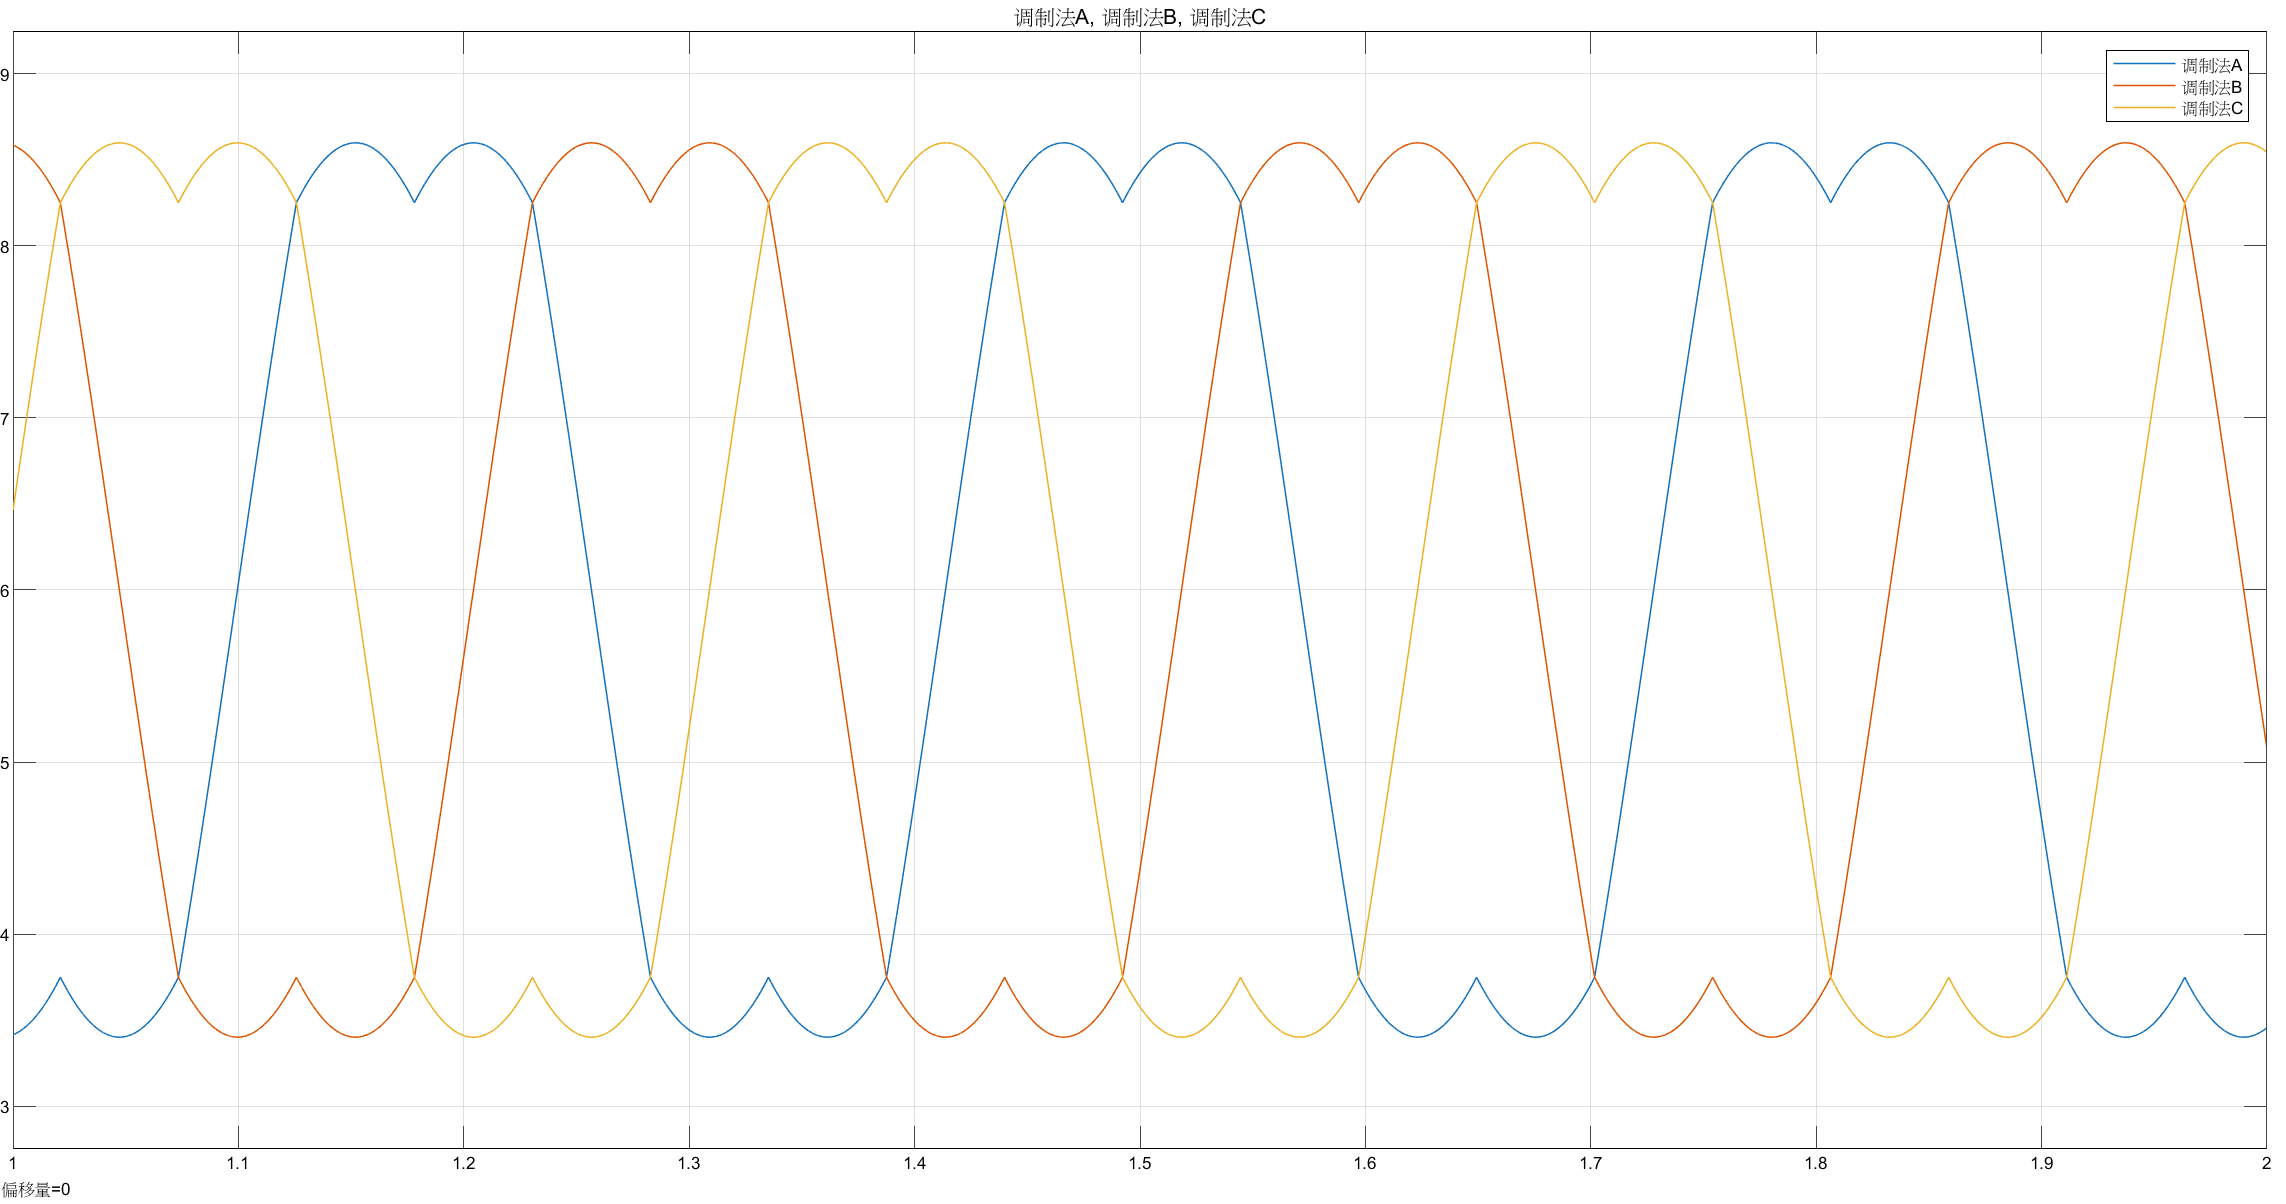
\includegraphics[width=0.8\textwidth]
    {图片/SVPWM电压波形.png}
    \caption{SVPWM电压波形}
    \label{fig:SVPWM电压}
\end{figure}

可以发现SVPWM波形为类马鞍波。若以SPWM调制的正弦波为基波，则SVPWM是在
正弦基波基础上叠加了一个基波频率为正弦基波频率三倍的波形。
为了便于观察，取A相电压波形，将直接通过克拉克-帕克逆变换的原始波形、
通过SVPWM调制后的相电压波形（去除直流分量）相比，并且用SVPWM调制波形
减去原始波形，观察注入波形的样式，
如下图\ref{fig:A相电压波形}所示。
\begin{figure}[H]
    \centering
    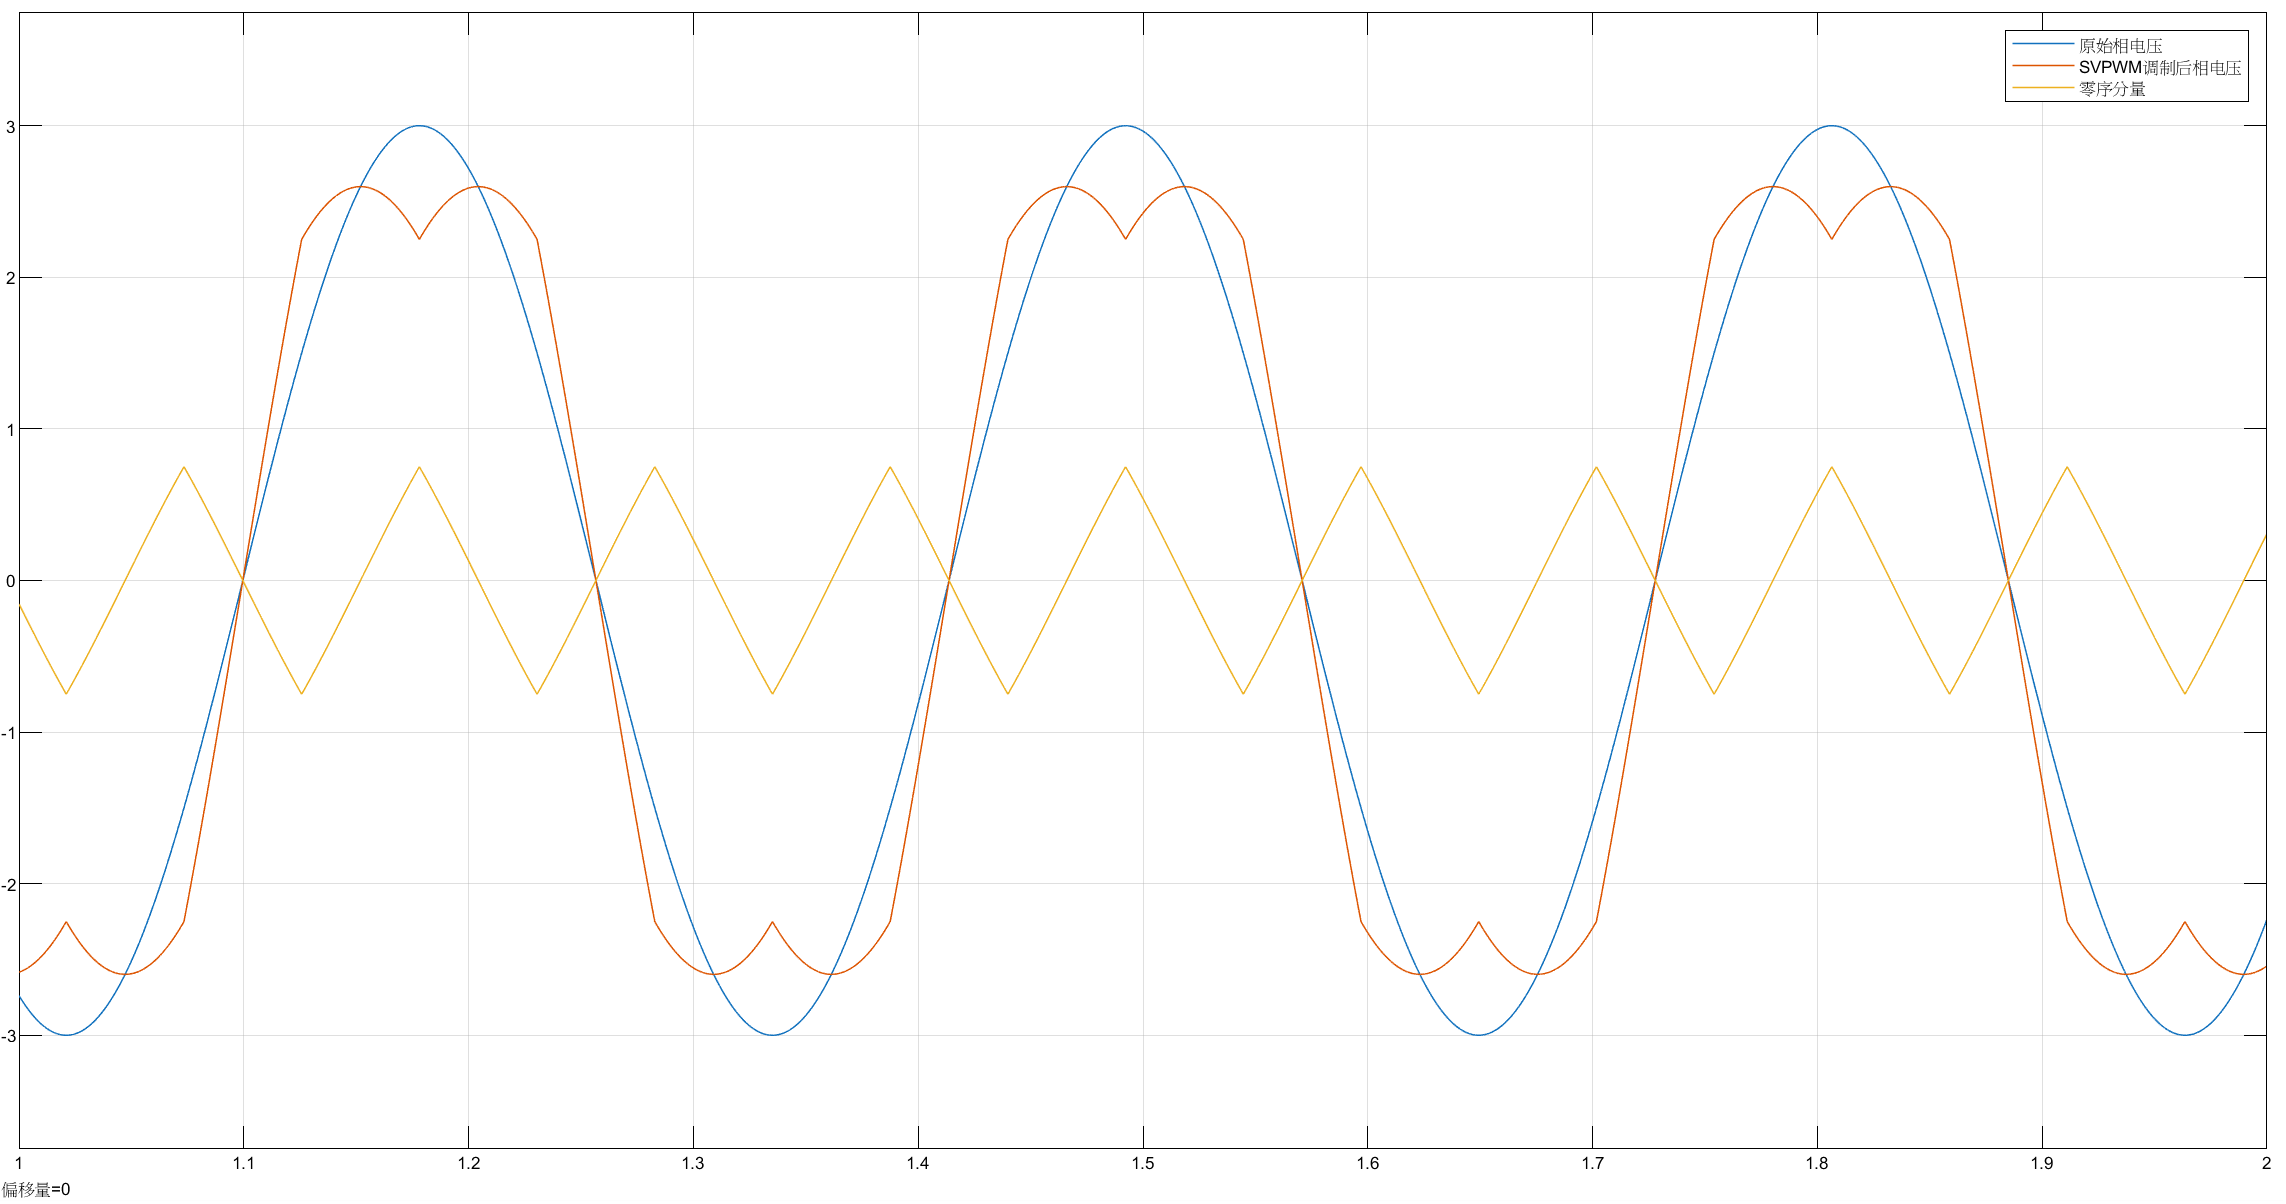
\includegraphics[width=0.8\textwidth]
    {图片/A相电压波形.png}
    \caption{A相电压波形}
    \label{fig:A相电压波形}
\end{figure}

SVPWM调制通过在基波基础上注入三倍频率的三角波实现了
电压利用率的提高，这是SVPWM电压利用率远超SPWM的关键所在。
由于该三角波在相电压中注入且基波频率恰好是正弦波频率的三倍，
因此在线电压中会相互抵消，使得线电压波形仍为正弦波。
由于该三角波注入没有影响线电压谐波，所以将该三角波称为零序分量。

零序分量\(U_{\mathrm{0}}\)与克拉克-帕克逆变换得到的三相电压波形如下图
\ref{fig:原始相电压波形与零序分量波形}所示。
可以发现，零序分量在自然换相点达到极值，在任意一相过零点归零，
并且全程线性变化。
\begin{figure}[H]
    \centering
    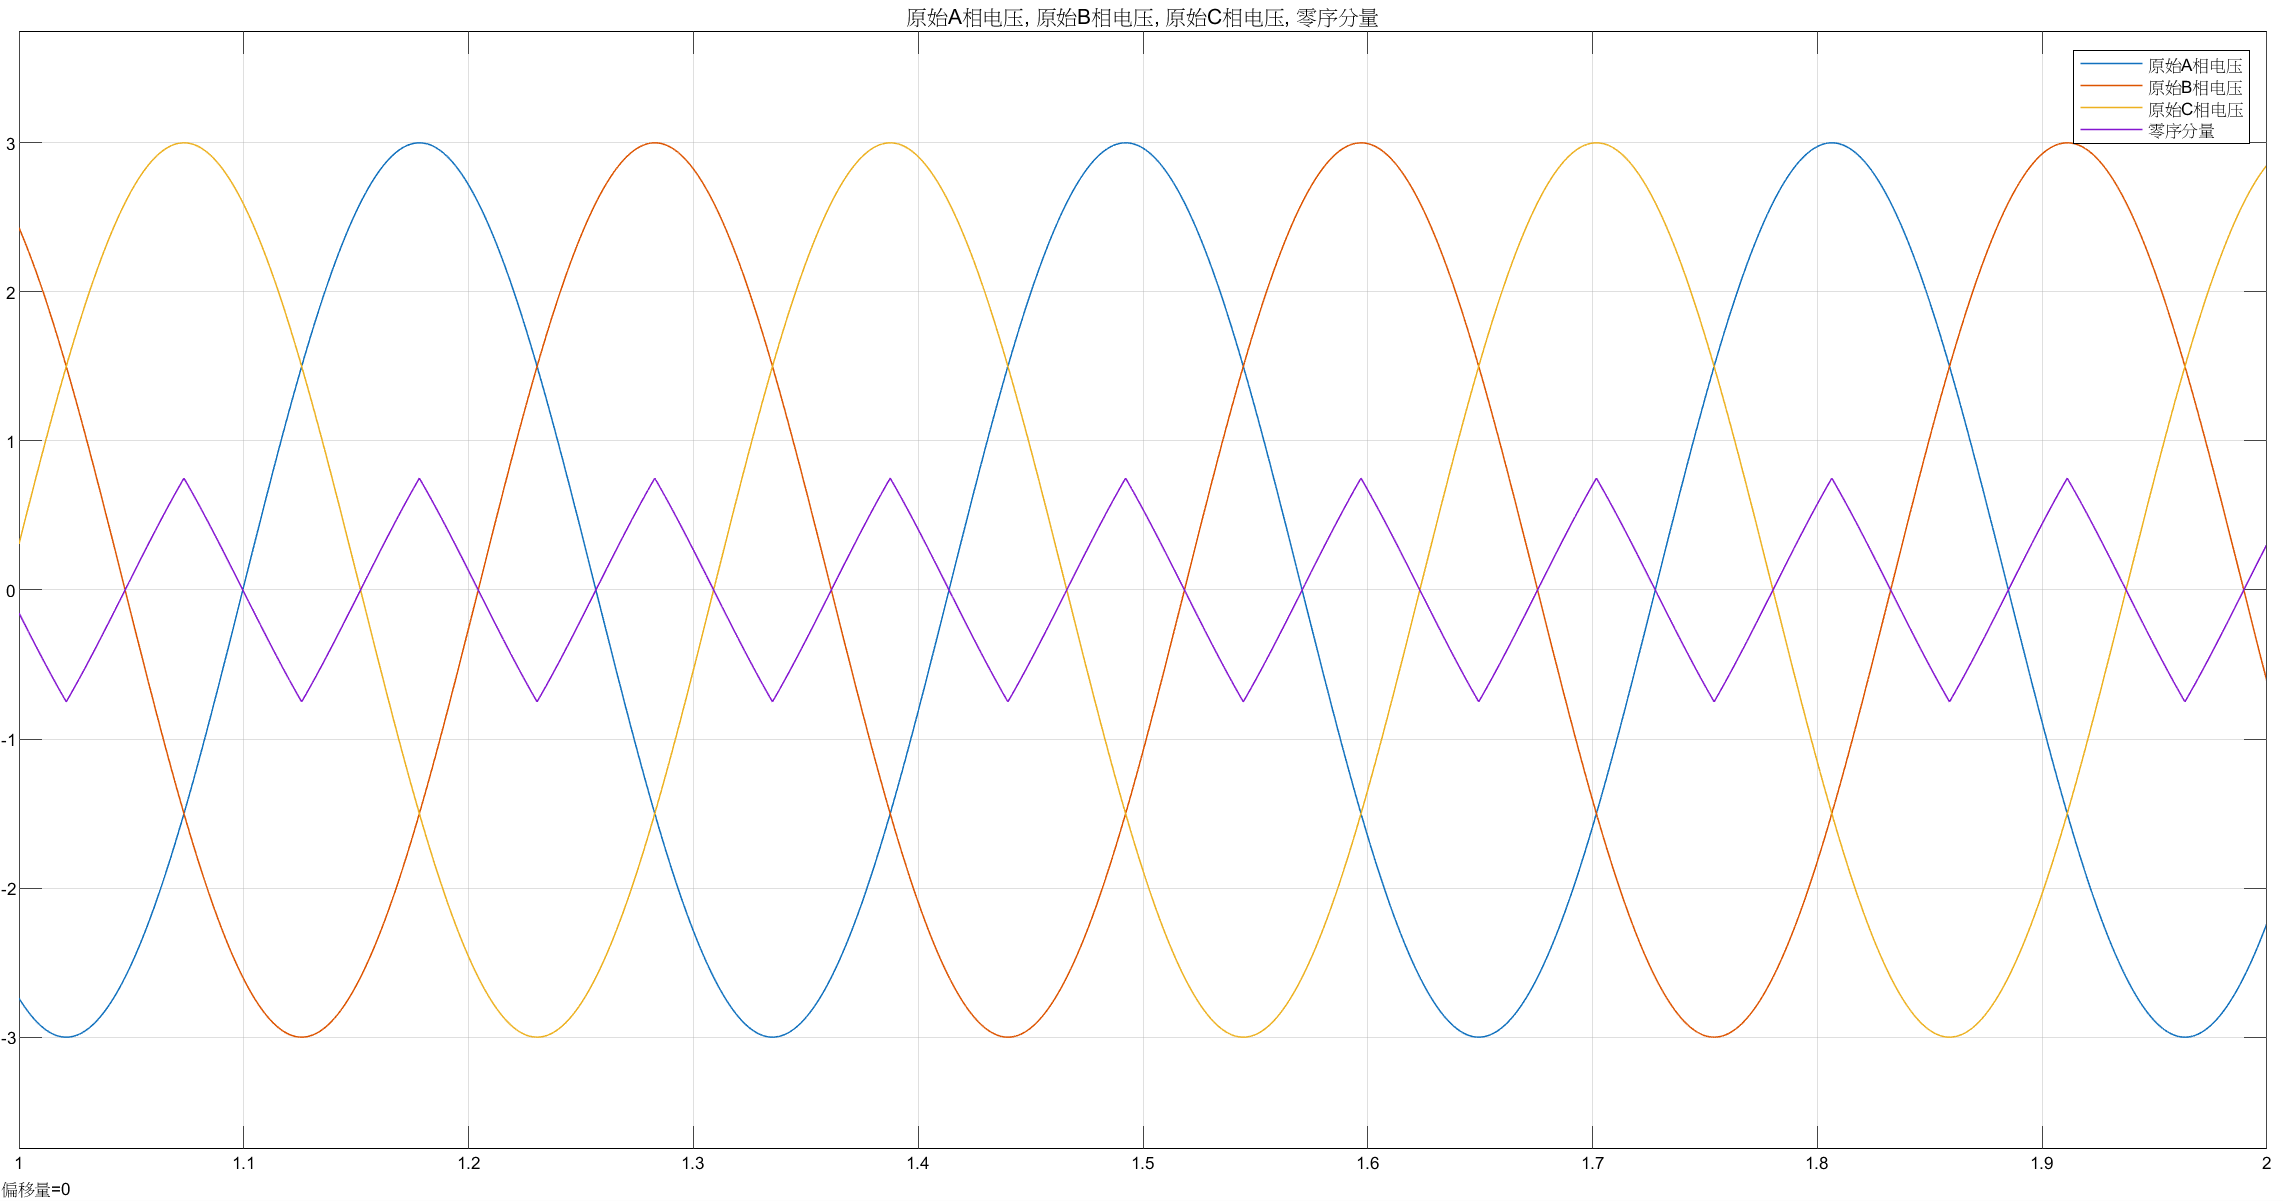
\includegraphics[width=0.8\textwidth]
    {图片/原始相电压波形与零序分量波形.png}
    \caption{原始相电压波形与零序分量波形}
    \label{fig:原始相电压波形与零序分量波形}
\end{figure}

设期望的\(U_{\mathrm{d}},U_{\mathrm{q}}\)经过克拉克-帕克逆变换得到的三相原始相电压为
\(U_{\mathrm{a}},U_{\mathrm{b}},U_{\mathrm{c}}\)。
注入零序分量\(U_{\mathrm{0}}\)后，调制相电压为：
\begin{equation}
    \begin{cases}
        U_{\mathrm{a}}' = U_{\mathrm{a}} + U_{\mathrm{0}}\\
        U_{\mathrm{b}}' = U_{\mathrm{b}} + U_{\mathrm{0}}\\
        U_{\mathrm{c}}' = U_{\mathrm{c}} + U_{\mathrm{0}}   
    \end{cases}
    \label{eq:注入后相电压}
\end{equation}

可以发现，零序分量注入前后线电压维持恒定：
\begin{equation*}
    \begin{cases}
        U_{\mathrm{ab}}' = U_{\mathrm{a}}' - U_{\mathrm{b}}'
        = U_{\mathrm{a}} - U_{\mathrm{b}} = U_{\mathrm{ab}}\\
        U_{\mathrm{bc}}' = U_{\mathrm{b}}' - U_{\mathrm{c}}'
        = U_{\mathrm{b}} - U_{\mathrm{c}} = U_{\mathrm{bc}}\\
        U_{\mathrm{ca}}' = U_{\mathrm{c}}' - U_{\mathrm{a}}'
        = U_{\mathrm{c}} - U_{\mathrm{a}} = U_{\mathrm{ca}}
    \end{cases}
\end{equation*}

因此无论\(U_{\mathrm{0}}\)取何值，线电压波形始终保持不变。
也就是说，在线性调制的前提下，零序分量注入与否不影响实际的电机运行
\footnote{电机运行主要取决于线电压而不是相电压。}。但零序分量注入后，
相同线电压需要的相电压幅值降低，相当于扩大了线性调制区间。
为保证线性调制（不进入过调制区），调制后的三相相电压必须限制在
直流母线电压范围内：
\begin{equation*}
    -\cfrac{U_{\mathrm{dc}}}{2} \le U_{\mathrm{a}}',U_{\mathrm{b}}',U_{\mathrm{c}}'
    \le \cfrac{U_{\mathrm{dc}}}{2}
\end{equation*}

记三相原始电压的最大值和最小值分别为
\begin{equation*}
    \begin{cases}
        U_{\mathrm{\max}} = \max(U_{\mathrm{a}},U_{\mathrm{b}},U_{\mathrm{c}})\\
        U_{\mathrm{\min}} = \min(U_{\mathrm{a}},U_{\mathrm{b}},U_{\mathrm{c}})
    \end{cases}
\end{equation*}

则上述电压范围约束等价于对调制后最大相电压和最小相电压的要求：
\begin{equation*}
    \begin{cases}
        U_{\mathrm{\min}} + U_{\mathrm{0}} \ge -\cfrac{U_{\mathrm{dc}}}{2}\\[8pt]
        U_{\mathrm{\max}} + U_{\mathrm{0}} \le \cfrac{U_{\mathrm{dc}}}{2}
    \end{cases}
\end{equation*}

满足上式的\(U_{\mathrm{0}}\)有无穷多个，
而SVPWM选择的策略为居中对称，
令调制后最大相电压到上边界的电压裕量\(\cfrac{U_{\mathrm{dc}}}{2}-(U_{\mathrm{\max}}+U_{\mathrm{0}})\)
与最小相电压到下边界的电压裕量\((U_{\mathrm{\min}}+U_{\mathrm{0}})-(-\cfrac{U_{\mathrm{dc}}}{2})\)
保持相等，即：
\begin{equation*}
    \cfrac{U_{\mathrm{dc}}}{2} - (U_{\mathrm{\max}} + U_{\mathrm{0}})
    = (U_{\mathrm{\min}} + U_{\mathrm{0}}) + \cfrac{U_{\mathrm{dc}}}{2}
\end{equation*}

化简得：
\begin{equation}
    U_{\mathrm{0}} = -\cfrac{1}{2}(U_{\mathrm{\max}} + U_{\mathrm{\min}})
    \label{eq:零序分量表达式}
\end{equation}

因此就可以得到计算法的三相占空比表达式：
\begin{equation}
    \begin{cases}
        D_{\mathrm{A}} = \cfrac{1}{2} +\cfrac{U_{\mathrm{0}}+U_{\mathrm{a}}}{U_{\mathrm{dc}}}\\
        D_{\mathrm{B}} = \cfrac{1}{2} +\cfrac{U_{\mathrm{0}}+U_{\mathrm{b}}}{U_{\mathrm{dc}}}\\
        D_{\mathrm{C}} = \cfrac{1}{2} +\cfrac{U_{\mathrm{0}}+U_{\mathrm{c}}}{U_{\mathrm{dc}}}
    \end{cases}
    \label{eq:三相占空比表达式}
\end{equation}

式\eqref{eq:零序分量表达式}即为SVPWM零序分量的解析表达式。相关的波形示意如下图所示。
\begin{figure}[H]
    \centering
    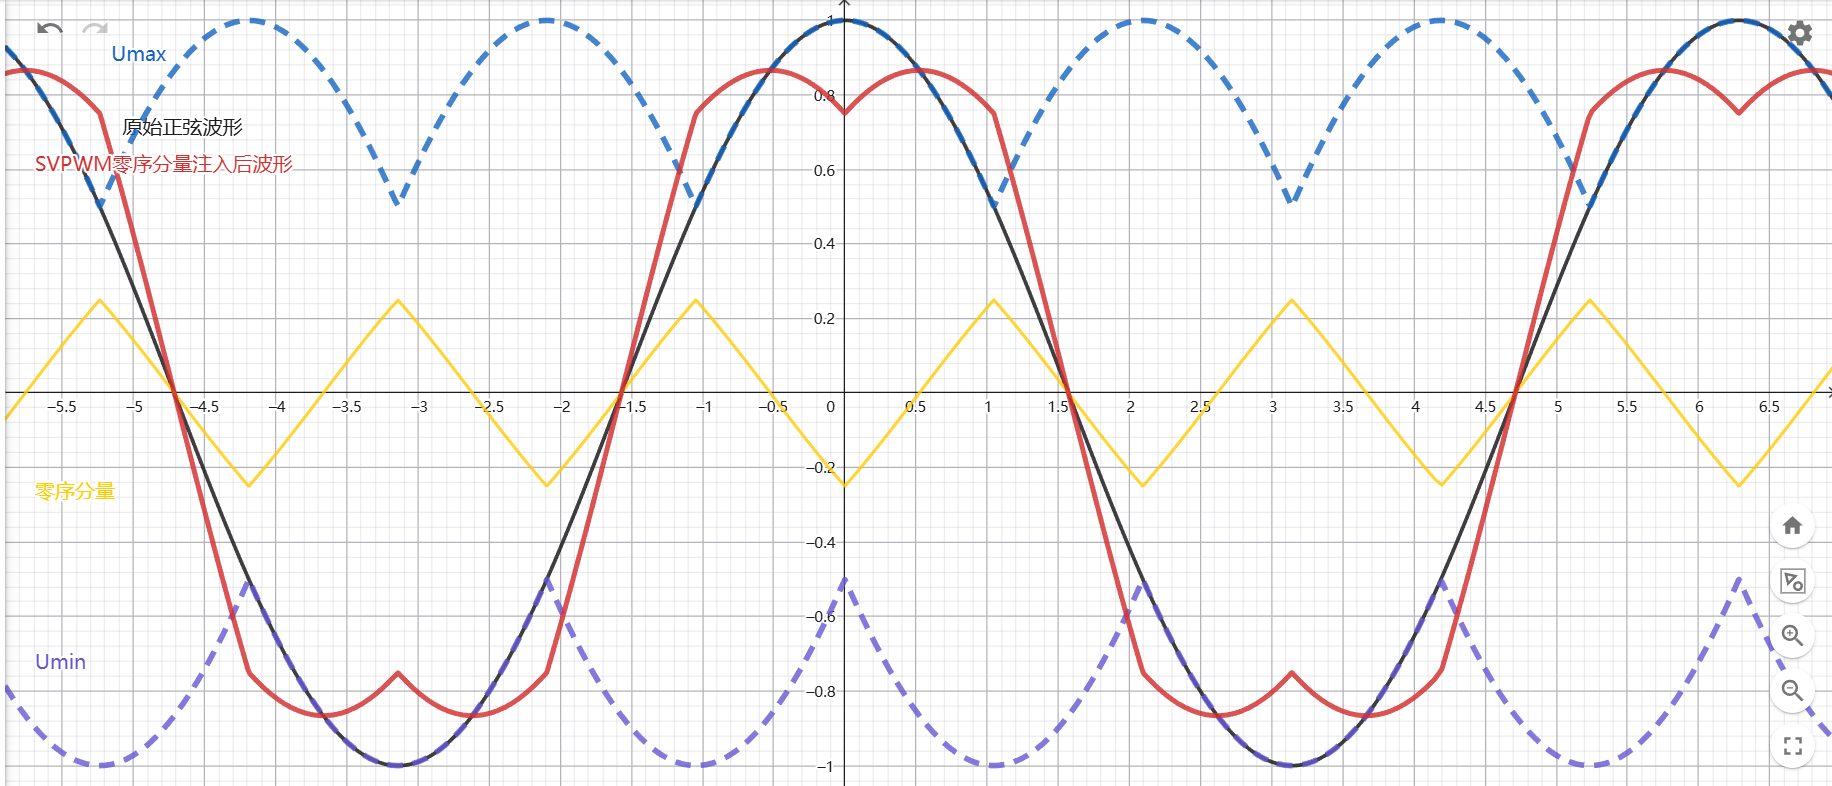
\includegraphics[width=0.8\textwidth]
    {图片/零序分量计算相关波形.png}
    \caption{零序分量计算相关波形示意}
    \label{fig:零序分量计算相关波形示意}
\end{figure}

接下来以第I扇区为例，证明\eqref{eq:零序分量表达式}零序分量注入的结果与第\ref{sec:SVPWM调制法}节中给出的调制法结果一致。
根据调制法中间步骤，中间变量满足：
\begin{equation*}
    \begin{cases}
        A_0 = U_{\mathrm{\beta}}\\
        A_1 = \cfrac{\sqrt{3}}{2}U_{\mathrm{\alpha}} - \cfrac{1}{2}U_{\mathrm{\beta}}\\
        A_2 = -\cfrac{\sqrt{3}}{2}U_{\mathrm{\alpha}} - \cfrac{1}{2}U_{\mathrm{\beta}}\\
        K = \cfrac{\sqrt{3}T_{\mathrm{s}}}{U_{\mathrm{dc}}}
    \end{cases}
\end{equation*}

由表\ref{tab:基本矢量作用时间计算表(TU1,TU2表示)}可知，
第I扇区有\(T_{\mathrm{U1}} = KA_1\)，\(T_{\mathrm{U2}} = KA_0\)，
而\(T_0=T_{\mathrm{s}}-T_{\mathrm{U1}}-T_{\mathrm{U2}}\)，
代入占空比定义可得：
\begin{equation*}
    \begin{cases}
        D_0=\cfrac{T_0}{2T_{\mathrm{s}}}=\cfrac{1}{2}(1-\cfrac{\sqrt{3}A_1}{U_{\mathrm{dc}}}
        -\cfrac{\sqrt{3}A_0}{U_{\mathrm{dc}}})\\
        D_1=D_0+\cfrac{T_{\mathrm{U2}}}{T_{\mathrm{s}}}=\cfrac{1}{2}(1-\cfrac{\sqrt{3}A_1}{U_{\mathrm{dc}}}
        +\cfrac{\sqrt{3}A_0}{U_{\mathrm{dc}}})\\
        D_2=D_1+\cfrac{T_{\mathrm{U1}}}{T_{\mathrm{s}}}=\cfrac{1}{2}(1+\cfrac{\sqrt{3}A_1}{U_{\mathrm{dc}}}
        +\cfrac{\sqrt{3}A_0}{U_{\mathrm{dc}}})
    \end{cases}
\end{equation*}

由表\ref{tab:三相占空比计算表}，第I扇区三相占空比分配为
A相\(D_2\)、B相\(D_1\)、C相\(D_0\)。
相较于虚拟中性点\(\cfrac{1}{2}U_{\mathrm{dc}}\)的调制相电压由占空比决定：
\begin{equation*}
    \begin{cases}
        U_{\mathrm{a,M}}' = (D_{\mathrm{A}}-\cfrac{1}{2})U_{\mathrm{dc}}=(D_{2}-\cfrac{1}{2})U_{\mathrm{dc}}
        =\cfrac{\sqrt{3}}{2}(A_0 + A_1)\\
        U_{\mathrm{b,M}}' = (D_{\mathrm{B}}-\cfrac{1}{2})U_{\mathrm{dc}}=(D_{1}-\cfrac{1}{2})U_{\mathrm{dc}}
        =\cfrac{\sqrt{3}}{2}(A_0 - A_1)\\
        U_{\mathrm{c,M}}' = (D_{\mathrm{C}}-\cfrac{1}{2})U_{\mathrm{dc}}=(D_{0}-\cfrac{1}{2})U_{\mathrm{dc}}
        =\cfrac{\sqrt{3}}{2}(-A_0 - A_1)
    \end{cases}
\end{equation*}

另一边，根据克拉克变换\eqref{eq:克拉克变换}，原始三相电压可以用逻辑向量\(A_0,A_1\)表示为：
\begin{equation*}
    \begin{cases}
        U_{\mathrm{a}} = U_{\mathrm{\alpha}}
        = \cfrac{1}{\sqrt{3}}(2A_1 + A_0)\\
        U_{\mathrm{b}} = -\cfrac{1}{2}U_{\mathrm{\alpha}} + \cfrac{\sqrt{3}}{2}U_{\mathrm{\beta}}
        = \cfrac{1}{\sqrt{3}}(A_0-A_1)\\
        U_{\mathrm{c}} = -\cfrac{1}{2}U_{\mathrm{\alpha}} - \cfrac{\sqrt{3}}{2}U_{\mathrm{\beta}}
        = \cfrac{1}{\sqrt{3}}(-A_1-2A_0)
    \end{cases}
\end{equation*}

在第I扇区，由扇区判断条件易知\(U_{\mathrm{a}}>U_{\mathrm{b}}>U_{\mathrm{c}}\)，
即\(U_{\mathrm{\max}}=U_{\mathrm{a}}\)，\(U_{\mathrm{\min}}=U_{\mathrm{c}}\)。
将上式代入零序分量公式
\eqref{eq:零序分量表达式}可得：
\begin{equation*}
    U_{\mathrm{0}} = -\cfrac{U_{\mathrm{a}} + U_{\mathrm{c}}}{2} = \cfrac{1}{2\sqrt{3}}(A_0-A_1)
\end{equation*}

将原始相电压与零序分量叠加，得到计算法在第I扇区的调制相电压：
\begin{equation*}
    \begin{cases}
        U_{\mathrm{a,C}}'=U_{\mathrm{a}}+U_{\mathrm{0}}
        =\cfrac{1}{2\sqrt{3}}(3A_1+3A_0)=\cfrac{\sqrt{3}}{2}(A_0 + A_1)=U_{\mathrm{a,M}}'\\
        U_{\mathrm{b,C}}'=U_{\mathrm{b}}+U_{\mathrm{0}}
        =\cfrac{1}{2\sqrt{3}}(3A_0-3A_1)=\cfrac{\sqrt{3}}{2}(A_0 - A_1)=U_{\mathrm{b,M}}'\\
        U_{\mathrm{c,C}}'=U_{\mathrm{c}}+U_{\mathrm{0}} 
        =\cfrac{1}{2\sqrt{3}}(-3A_1-3A_0)=\cfrac{\sqrt{3}}{2}(-A_0 - A_1)=U_{\mathrm{c,M}}'\\
    \end{cases}
\end{equation*}

可以发现调制法和计算法结果一致。其余五个扇区证明同理。通过SVPWM计算法，大大省略了调制法需要的查表运算，无需
程序分支，只需要按照公式\eqref{eq:零序分量表达式}
和\eqref{eq:三相占空比表达式}计算即可，更加适合实时控制场合。
